%!TEX root=masterproef.tex

\subsection{Detecteren van anomalie\"en}
\label{subsection:anomaly}

Een anomalie is een afwijking van een normaal verloop van gebeurtenissen of
iets of iemands gedrag. Een knoop uit een DSN heeft een redelijk eenvoudig en
constante levensloop. Typisch zal een knoop op regelmatige tijdstippen
\emph{wakker worden}, waarden opmeten aan de hand van zijn sensoren en deze
waarden doorsturen naar een centrale locatie. Verder zal een knoop, als
onderdeel van het netwerk, tevens zulke waarden van andere knopen doorsturen.
Dit patroonmatige gedrag kan ge\"identificeerd worden en in een model verwerkt
worden. Op basis van zulk een model kan vervolgens nagegaan worden of de acties
van een knoop op een gegeven moment in lijn zijn met het model of dat er sprake
is van een anomalie.

Zulk een afwijking van het verwachte gedrag kan wijzen op veranderingen van
buitenaf. Deze kunnen op hun beurt veroorzaakt zijn door een aanval op het
netwerk. Aangezien we niet alle communicatie van en naar knopen kunnen
onderscheppen en eventuele aanvallen kunnen detecteren, kunnen
anomaliegebaseerde dectectiemechanismen helpen om op basis van neveneffecten
toch aanvallen te detecteren, of althans toch de gevolgen ervan.

\subsubsection*{Anomali\"en, afwijkingen, aberraties}
\label{subsubsection:outlier}

\citep{zhang2010outlier} is een excellent overzicht van methoden om anomali\"en,
afwijkingen of aberraties (Engels: \emph{outliers}) te detecteren in een reeks
van metingen. Het belicht enerzijds de fundamentele technieken die ter
beschikking staan om deze aberraties op te merken maar tracht ook een
classificatie en taxonomie op te stellen hiervoor.

De auteurs stellen dat het detecteren van afwijkingen behoort tot het domein
van \emph{datamining} en dat het in die context reeds uitvoerig onderzocht is,
evenals binnen disciplines as statistiek, machinaal leren, informatie
theorie,\dots. Aangezien het kunnen uitsluiten van afwijkingen de verwerking
van de overblijvende meetresultaten sterk positief be\"invloed is het in het
kader van DSN uitermate interessant.

Toch kan eerder onderzoek opnieuw niet eenvoudig toegepast worden in het kader
van DSN. De beperkte middelen van de sensorknoop schrappen al veel van de
klassieke oplossingen die bv. gecentraliseerd werken. De overdaad aan
communicatie die nodig is om voldoende gegevens te centraliseren voor
verwerking is niet realistisch in het kader van een DSN. Ook zijn veel van de
algoritmen typisch niet ontwikkeld met de beperkte rekenmogelijkheden van
sensorknopen. De conclusie is dat er een balans moet gevonden worden tussen de
mogelijkheden van datamining algoritmen voor het detecteren van afwijkingen en
de verhouding van hun noden ten opzichte van de middelen van de knopen.

Figuur \ref{fig:outlier-detection-taxonomy} geeft een overzicht van de
taxonomie die de auteurs opstelden specifiek voor DSN.

\begin{figure}[ht]
  \centering
  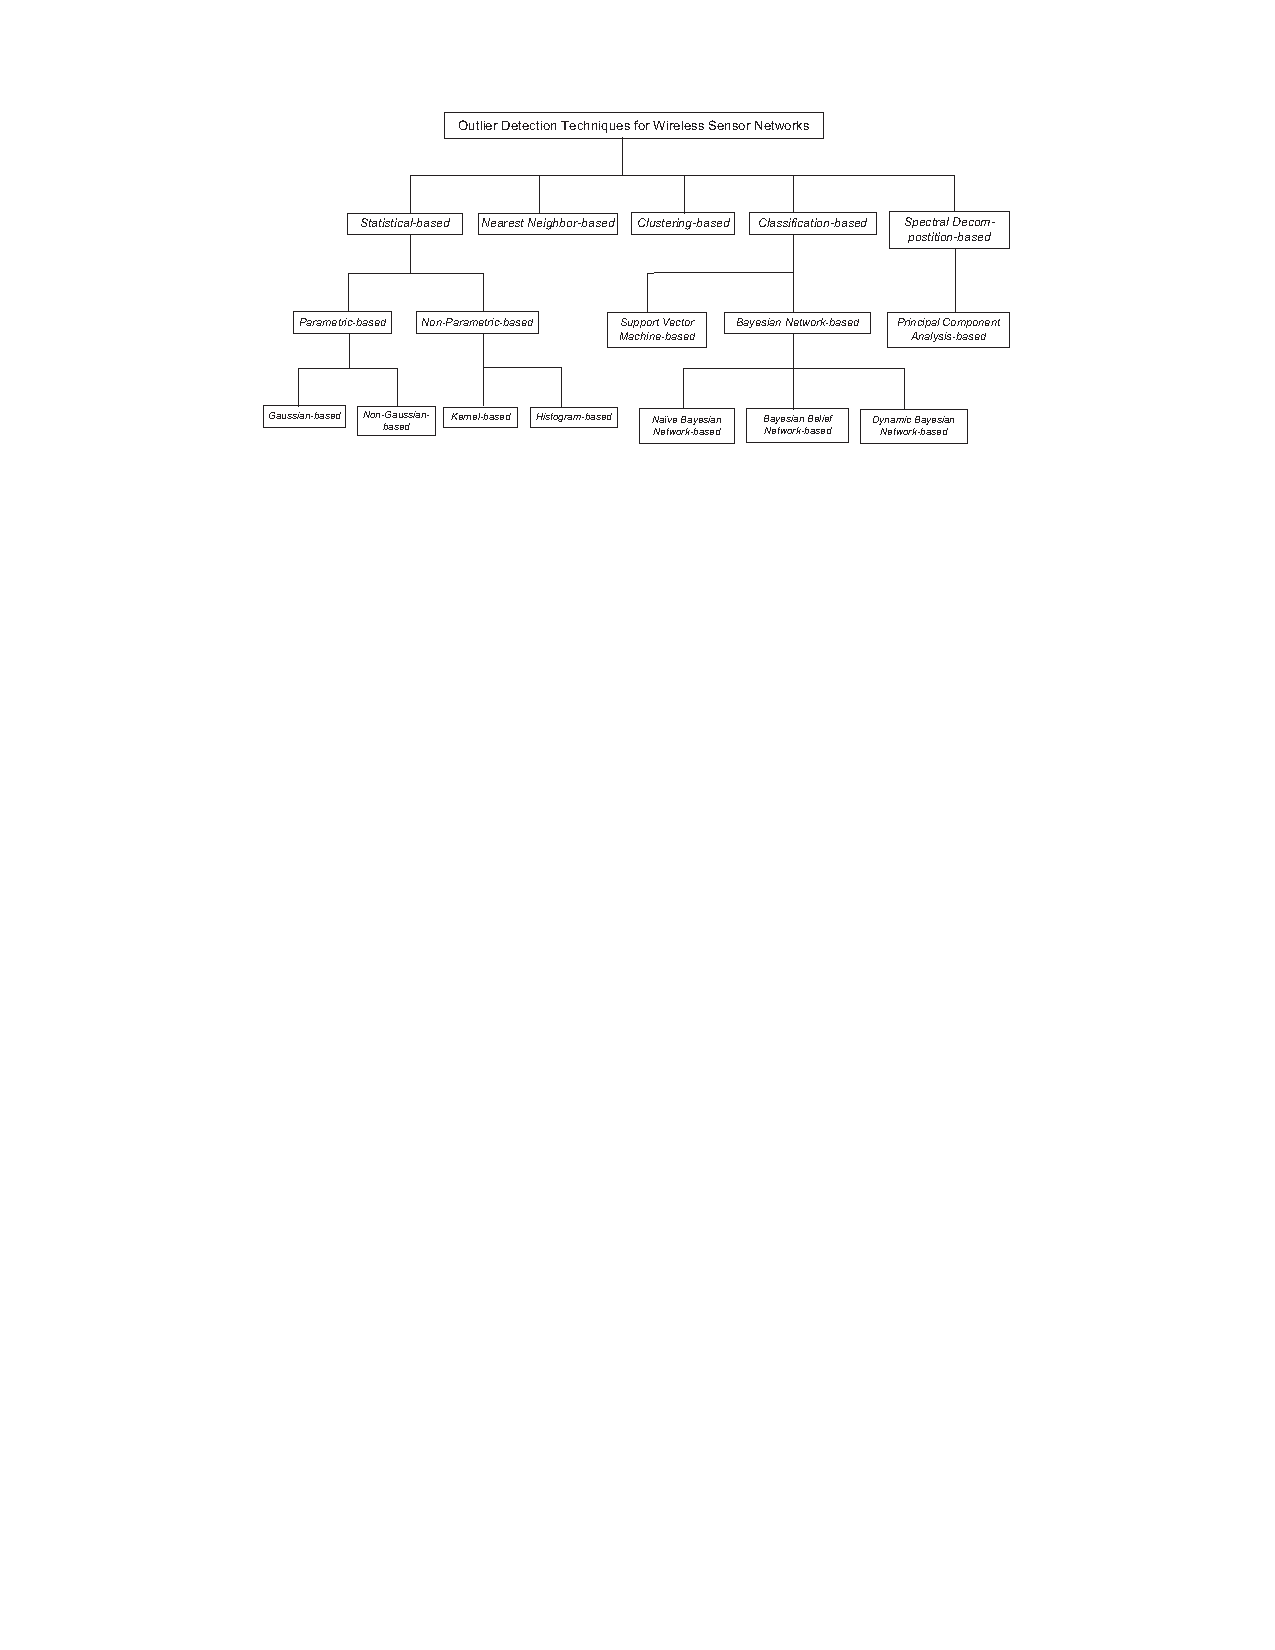
\includegraphics[width=\linewidth]{resources/outlier-detection-taxonomy.pdf}
  \caption[Taxonomie voor detectie van afwijkingen.]{Een taxonomie voor technieken om afwijkingen te detecteren. \citep{zhang2010outlier}}
  \label{fig:outlier-detection-taxonomy}
\end{figure}

Verder worden ook enkele tekortkomingen van detectietechnieken besproken. Zo
wordt opgemerkt dat dikwijls gekeken wordt naar losse meetwaarden, terwijl een
sensorknoop meerdere sensorwaarden kan aanbieden. Het gebeurt echter vaak dat
er nauwelijks een anomalie kan opgemerkt worden wanneer men naar \'e\'en enkele
meetwaarde kijkt, maar wanneer men de verschillende meetwaarden samen bekijkt,
dat er zich opvallende aberraties kunnen voordoen.

Wanneer naburige sensorknopen worden beschouwd om relaties tussen knopen te
gebruiken om meetwaarden af te wegen ten opzichte van elkaar, blijkt dat er
dikwijls problematische keuzes gemaakt worden met betrekking tot de reikwijdte
van de buurt of in het geval van tijd tot de grootte van de voortschrijdende
tijdspanne die in beschouwing wordt genomen.

Gerelateerd hieraan is ook de foute veronderstelling dat knopen een vaste
locatie hebben en niet verplaatst worden. Maar ook het manueel kiezen van
drempelwaarden en het vaag defini\"eren van het verschil tussen gebeurtenissen
en fouten leidt dikwijls tot problemen.

De auteurs bieden ook een overzicht van eisen die gesteld moeten worden aan
detectiealgoritmes voor anomali\"en. Ofschoon er weinig verrassingen tussen
zitten, is het toch een interessante en nuttige lijst omdat deze duidelijke
eisen en impliciete voorwaarden stelt voor goede algoritmes. Indien mogelijk
willen we deze eigenschappen als constructieve beperkingen opnemen in ons
raamwerk.

\begin{itemize}

  \item Verwerking van gegevens moet gedistribueerd kunnen gebeuren, om zo de
  communicatiekost laag te houden.

  \item Het algoritme moet kunnen werken op basis van een continue stroom aan
  gegevens.

  \item De detectiegraad moet hoog zijn en de foutenmarge laag.

  \item Het algoritme moet zich zonder manuele interventie kunnen configureren
  en later ook opereren omdat het moeilijk is op voorhand een stabiele
  configuratie voor een DSN op te stellen.

  \item Als een sensorknoop over meerdere sensoren beschikt, moeten de
  resultaten ook samen bekeken worden.

  \item Schaalbaarheid is een belangrijke factor aangezien sensorknopen soms in
  groten getale worden ingezet.

  \item Algoritmes moeten rekening houden met de afhankelijkheden tussen de
  eigenschappen van de meetwaarden, als ook met de ruimte- en tijd-correlaties
  tussen de observaties van naburige knopen.

\end{itemize}

\subsubsection*{Neurale netwerken}
\label{subsubsection:neuralnetworks}

Wanneer men denkt aan het vastleggen van een patroon en het controleren of een
bepaalde situatie voldoet aan dat patroon wordt in informatiecakringen ook snel
verwezen naar neurale netwerken. Neurale netwerken kunnen immers
\emph{getraind} worden door middel van een aantal goede (en slechte)
voorbeelden, waarna nieuwe voorbeelden kunnen gecatalogeerd worden als ook goed
of slecht. De complexiteit van het bepalen van deze beslissing is typisch
redelijk eenvoudig en lijkt zich daarom uitermate goed te lenen voor het
detecteren van anomalie\"en door sensorknopen.

In \citep{ramesh2012wireless} volgen de auteurs deze denkpiste, maar stellen
tevens dat er betere methoden bestaan. Ze trachten twee specifieke aanvallen
het hoofd te bieden: DoS en passieve informatie vergaring en vergelijken
hierbij een aanpak op basis van een neuraal netwerk en hun eigen aanpak op
basis van encryptie op basis van symmetrische sleutels.

Hun oplossing maakt gebruik van de technische aspecten van het verzenden van
berichten over het draadloze medium. Het principe van een draadloze
radioverbinding laat slechts \'e\'en zender tegelijkertijd toe. In sectie
\ref{subsubsection:mac} belichtten we reeds kort deze principes en de mogelijk
problemen die hierbij kunnen ontstaan indien deelnemers aan het netwerk zich
niet houden aan de afspraken omtrent het opstarten van communicatie. Daarom
voorzien de meeste DSN een zgn. \emph{carrier sens multiple access with
collision avoidance} (CSMA/CA) mechanisme. Dit berust op het uitwisselen van
\emph{ready to send} (RTS) en \emph{clear to send} (CTS) berichten.

Wanneer een knoop gegevens wil versturen zal het dit aankondigen met een RTS
pakket en dus aangeven dat het klaar staat om deze gegevens te versturen. Een
andere knoop die dit pakket ontvangt zal antwoorden met een CTS pakket en zo
aan de vragende knoop bevestigen dat het zijn beurt is om zijn gegevens te
verzenden. Zowel het RTS pakket als het CTS pakket zorgen er voor dat andere
knopen wachten met het verzenden van informatie en uiteindelijk zal \'e\'en CTS
pakket toekomen bij de oorspronkelijke initiator van het RTS pakket, waarna
deze zijn gegevens kan versturen met de garantie dat andere knopen het medium
niet zullen verstoren.

Op basis van eerder onderzoek stellen de auteurs dat het mogelijk is om een DoS
te detecteren op basis van drie parameters: $R_c$ is het aantal conflicten
(Engels: \emph{collisions}) die zich voordoen bij een knoop gedurende een
seconde, $R_t$ is het aantal RTS pakketten die succesvol ontvangen worden door
een knoop per seconde en $T_w$ die de gemiddelde wachttijd weergeeft van een
pakket in de MAC buffer voor het effectief verzonden wordt.

Voor hun eigen simulatie gebruiken de auteurs alleen de waarden van $R_c$ em
$R_t$. In hun voorbereidend werk bleek $T_w$ geen invloed te hebben. Ze
gebruikten een vrij standaard \emph{meerlagig percetron} (MLP), wat algemeen
beschouwd wordt als het populairste neurale netwerk om te leren onder toezicht.

Naast de aanpak op basis van neurale netwerken, voorzien de auteurs tevens een
oplossing op basis van encryptie door middel van symmetrische sleutels. Ze gaan
er van uit dat een aanvaller geen weet heeft van het gebruik van een 8 bits
gedeelde sleutel en dat hij daarom nooit op een correcte manier gegevens over
het netwerk zal kunnen versturen en daarom ook nooit succesvol een DoS zal
kunnen initi\"eren noch passief (nuttige) gegevens kunnen verzamelen.

Deze veronderstellingen zijn op zijn minst na\"ief. Zowel de beperkte grootte
van de sleutel als de veronderstelling dat een aanvaller het gebruik van
encryptie niet zou kunnen achterhalen, wijzen op een inschattingsfout van de
onderzoekers in kwestie.

Hun werk toont echter wel aan dat een aanpak met neurale netwerken eenvoudig te
realiseren is en een valabele piste kan zijn om anomaliedetectie te doen.

\subsubsection*{Voorspellingen}
\label{subsubsection:predictions}

Waar neurale netwerken in staat zijn om op basis van voorbeelden een nieuwe
situatie te catalogeren, kan men aan de hand van een Markov model
voorspellingen doen over de toekomst.

Het is deze piste dat onderzocht wordt in \citep{zhijie2012intrusion}. Opnieuw
betreft het een poging om DoS aanvallen te detecteren. De bedoeling is dat
sensorknopen individueel bepalen of er een DoS aanval bezig is. Volgens de
auteurs is dit mogelijk aan de hand van een Markov model dat het netwerkverkeer
voorspelt.

Het model wordt zo geconstrueerd dat er een verband ontstaat tussen de toestand
van een knoop in relatie tot het tijdstip en de verwachtte hoeveelheid gegevens
die verstuurd zouden kunnen worden.

Het idee achter het artikel lijkt een mogelijke piste, maar omtrent veel
belangrijke details blijven echter zeer vaag, waardoor de volledige toedracht
van het algoritme niet eenduidig ingeschat kan worden. Zo wordt bv. nauwelijks
ingegaan op wat de toestand van een knoop juist bepaalt of hoe de
hoeveelheid gegevens die verstuurd kunnen worden wanneer een knoop zich in een
bepaalde toestand bevindt, bepaald wordt.
